%%% Laboratory	 Notes
%%% Template by Mikhail Klassen, April 2013
%%% Contributions from Sarah Mount, May 2014
\documentclass[a4paper]{tufte-handout}
\usepackage{tikz}

\newcommand{\workingDate}{\textsc{April $|$ 2022}}
\newcommand{\userName}{A.Belcaid}
\newcommand{\institution}{ENSA-Safi}

\usepackage{lab_notes}

\usepackage{hyperref}
\hypersetup{
    pdffitwindow=false,            % window fit to page
    pdfstartview={Fit},            % fits width of page to window
    pdftitle={Correction TD4},     % document title
    pdfauthor={A.Belcaid},         % author name
    pdfsubject={},                 % document topic(s)
    pdfnewwindow=true,             % links in new window
    colorlinks=true,               % coloured links, not boxed
    linkcolor=DarkScarletRed,      % colour of internal links
    citecolor=DarkChameleon,       % colour of links to bibliography
    filecolor=DarkPlum,            % colour of file links
    urlcolor=DarkSkyBlue           % colour of external links
}


\title{Solution TD 4}
\date{2022}

\begin{document}
\maketitle

\renewcommand{\P}{\mathbf{P}}

\section{Self-Inependence}

Soit $A$ un evenement de $\Omega$ et on suppose que $A$ est independant de $A$.

alors on aura que:

\begin{eqnarray*}
   \P(A \cap A) & = & \P(A)\cdot \P(A) \\
   \P(A)        & = & \P(A)^2
\end{eqnarray*}

Ce qui implique que $\P(A)= 1 $ ou $\P(A)=0$.

\hrule
\section{Modele conditionel}
on introduit les evenements 
\begin{itemize}
  \item $P = \{\text{\small Etudiant a prepare}\}$.
  \item $R = \{\text{\small Etudiant a reussi}\}$.
\end{itemize}
Selon l'enone on a:
\begin{equation*}
  \P(P) = p, \quad \P(R\;|\;P^c)= \frac{1}{2} = \P(R^c\;|\;P^c)\quad \text{ et }
  \P(R\;|\;P) = \alpha
\end{equation*}
La probabilite qu'on cherche est:

\begin{eqnarray*}
  P(P^c\;|\;R^c) &=& \frac{\P(P^c\cap T^c )}{\P(R^c)} \\[4pt]
                 &=& \frac{\P(R^c\;|\;P^c)\cdot \P(P^c)}{\P(R^c)}
\end{eqnarray*}
Maintenant on applique la loi de \textbf{probabilite totale} pour calculer
$\P(R^c)$.

\begin{eqnarray*}
  \P(R^c) &=& \P(P)\cdot\P(R^c|P) + \P(P^c)\cdot\P(R^c|P^c)\\
          &=& p(1-\alpha)  + \frac{1-p}{2}
\end{eqnarray*}

Ce qui nous donne que:

\begin{eqnarray*}
  \P(T^c\;|\; R^c) &=&  \frac{\P(R^c\;|\;P^c)\cdot \P(P^c)}{\P(R^c)}\\
                  & = & \frac{1-p}{1-p + 2(1-\alpha)p}
\end{eqnarray*}

\hrule

\section{Independence mutuelle}

\begin{enumerate}
  \item Demontrons que les trois evenements $A$, $B$ et $C$ sont independent
    deux a deux.\\

    On a $\P(B) = \P(C) = \frac{1}{2} $.\\

    Pour l'evenement $A$, on peut lister l'espace d'etat 
    \begin{equation*}
      \Omega=\{ (F,G), (F,F), (G,F), (G,G)\}
    \end{equation*}
    On endeduit que la probabilite de $A$ est $\P(A) = \frac{1}{2}$.

    On calcule alors les probabilite suivante:
    \begin{enumerate}
    \item $P(A\cap B) = \P(\{(F,F)\}) = \frac{1}{4} = \P(A)\cdot \P(B)$
    \item $P(A\cap C) = \P(\{(G,G)\}) = \frac{1}{4} = \P(A)\cdot \P(C)$
    \item $P(B\cap C) = \P(\{(F,G)\}) = \frac{1}{4} = \P(B)\cdot \P(C)$
    \end{enumerate}
    On conclut alors, que ces evenements sont independent \textbf{deux a deux}.
\item  Verifions si les trois sont mutuellement independents: 
  On as:

  \begin{equation*}
    \P(A\cap B\cap C)  =  P(B\cap C) = \frac{1}{4} \neq
    \P(A)\cdot\P(B)\cdot\P(C)
  \end{equation*}
\end{enumerate}

\hrule
\section{Fiabilite}

\begin{enumerate}
  \item Dans le premier diagramme:

    \begin{marginfigure}
      \begin{center}
      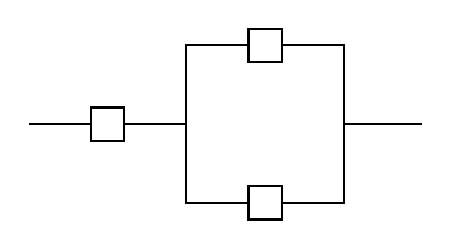
\begin{tikzpicture}[scale=1, transform shape]
       \node[draw, inner sep=0pt, minimum size=12pt, thick]  (A) at (0,0) {}; 
       \node[draw, inner sep=0pt, minimum size=12pt, thick]  (B) at (2,1) {}; 
       \node[draw, inner sep=0pt, minimum size=12pt, thick]  (C) at (2,-1) {}; 
       \path[draw,thick] (-1,0) -- (A) -- (1,0) --
         (1,1)--(B)--(3,1)--(3,0)--(4,0);

       \path[draw,thick] (-1,0) -- (A) -- (1,0) --
         (1,-1)--(C)--(3,-1)--(3,0)--(4,0);
      \end{tikzpicture}
      \end{center}
    \end{marginfigure}

    Pour ce diagramme, on calcule tout d'abord, la probabilite de l'unite en
    \textbf{paralelle}\footnote{Celle qui est a droite} soit en panne est les
    deux unites soit en panne. Ceci peut arriver avec une probabilite
    $(\frac{1}{3})\cdot (\frac{1}{3}) = \frac{1}{9}$. Ainsi cette unite sera
    fonctionnelle avec une probabilite $1 - \frac{1}{9} = \frac{8}{9}$.\\

    Maintenant Le systeme sera fonctionnel si celle a gauche et a droite sont
    fonctionnelles.\footnote{Puisqu'ils sont en serie}. Ceci peut arriver avec
    une probabilite:

    \begin{equation*}
      (\frac{8}{9})\cdot (\frac{2}{3}) = \frac{16}{27}
    \end{equation*}
  \item Pour le deuxieme diagramme:
    \begin{marginfigure}
        \begin{center}
        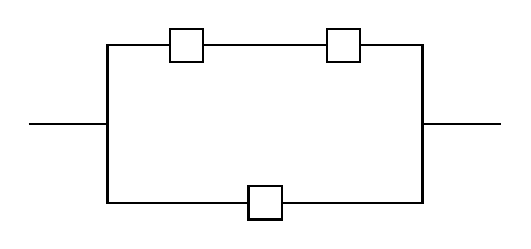
\begin{tikzpicture}[scale=1, transform shape]
       \node[draw, inner sep=0pt, minimum size=12pt, thick]  (A) at (1,1) {}; 
       \node[draw, inner sep=0pt, minimum size=12pt, thick]  (B) at (3,1) {}; 
       \node[draw, inner sep=0pt, minimum size=12pt, thick]  (C) at (2,-1) {}; 
       \path[draw,thick] (-1,0)--(0,0)--(0,1)--(A)--(B)--(4,1)--(4,0)--(5,0);
       \path[draw,thick] (-1,0)--(0,0)--(0,-1)--(C)--(4,-1)--(4,0)--(5,0);
        \end{tikzpicture}
        \end{center}
      \end{marginfigure}
      Il sera en panne si les deux entites\footnote{en haut en serie, et celle
      en bas}. sont en panne. 

      \begin{itemize}
        \item Celle en haut, elle sera en panne si \textbf{l'une des deux
          entites est en panne}.
          \begin{equation*}
            \P(\text{\small Up fonctionnelle})  = (\frac{2}{3})\cdot (\frac{2}{3}) = \frac{4}{9}
          \end{equation*}
        \item Ainsi la probabilite de panne sera:
          \begin{equation*}
            \P(\text{\small Up en panne})  = 1 - \frac{4}{9} = \frac{5}{9}
          \end{equation*}
        \item La probabilite que l'unite en bas soit en panne est 
          \begin{equation}
            \P(\text{\small Up en panne}) = \frac{1}{3}
          \end{equation}
      \end{itemize}
      Ainsi si on resume, on retrouve que le systeme sera en panne avec:

      \begin{equation*}
        \P(\text{\small{Systeme en panne}}) = (\frac{5}{9})\cdot(\frac{1}{3}) =
        \frac{5}{27}
      \end{equation*}
      Ce qui donne que la probablite qu'elle soit fonctionnelle est 
      \begin{equation*}
        \P(\text{\small{Systeme fonctionel}}) = 1 - \frac{5}{27} = \frac{22}{27}
      \end{equation*}
\end{enumerate}

\end{document}
